\documentclass[11pt]{article}

\usepackage[letterpaper, margin=1.45in]{geometry}

\usepackage{graphicx}
\usepackage{tikz}
\usepackage{float}
\usepackage{url}
\usepackage{epstopdf}
\usepackage{amssymb}
\usepackage{amsmath}
\usepackage{amsthm}
\usepackage{mathtools}

% layout
\usepackage{abstract}
\renewcommand{\abstractname}{}
\renewcommand{\absnamepos}{empty}

% paths
\graphicspath{{./bottleneck/}}

% style
\DeclareTextFontCommand{\emph}{\bfseries}

% defs
\def\E{\mathbb{E}}

% tikz
\def\layersep{1.5cm}

% worries
\usepackage{xcolor}
\newcommand\myworries[1]{\textcolor{red}{(#1)}}

\begin{document}
	
\begin{center}
{\LARGE On the Information Bottleneck} 
\end{center}

\begin{abstract}
The Information Bottleneck, introduced by Naftali Tishby et al. in 1999, formalizes the notion of an information-theoretic ``optimal'' representation in terms of the fundamental tradeoff between having a concise representation (compression) and one with good predictive power (accuracy). We draw connections to (1) minimal sufficient statistics, (2) the dynamics of stochastic gradient descent, (3) topologies of deep neural networks, (4) generalization bounds in learning theory, and (5) the formulation of variational auto-encoders.
\end{abstract}

\section{Information Theory}

Let $X, Y, Z$ denote discrete random variables. The Shannon \emph{entropy} captures the notion of the ``amount of information'' held in a random variable $X$:
\begin{equation}
H(X) = \E_p[-\log p(x)] = -\sum_{x} p(x) \log p(x).
\end{equation}
The \emph{conditional entropy} of $Y$ given $X$ quantifies the ``amount of information'' needed to describe the outcome of $Y$ given that the value of $X$ is known
\begin{equation}
H(Y\vert X) = -\sum_{x,y} p(x,y) \log p(y\vert x) = H(X,Y) - H(Y).
\end{equation}
The \emph{cross entropy} between $X$ and $Y$ of identical underlying set of events measures the average number of bits needed to identify an event drawn from the set
\begin{equation}
H(X, Y) = \E_p[-\log q(x)] = -\sum_{x} p(x)\log q(x) = H(P) + D_{KL}(P \,\rVert\, Q).
\end{equation}
The \emph{relative entropy} (Kullback-Leibler divergence) of $X$ with respect to $Y$ is a measure of how one distribution $P$ diverges from a expected distribution $Q$
\begin{equation}
D_{KL}(P \,\rVert\, Q)= \E_p[log \frac{p(x)}{q(x)}] = \sum_{x} p(x) \log \frac{p(x)}{q(x)} = H(P, Q) - H(P).
\end{equation}
The \emph{mutual information} quantifies the ``amount of information'', the average number of relevant bits, obtained about one random variable $X$, through the other random variable $Y$:
\begin{equation}
I(X;Y) = D_{KL}(p(x,y) \rVert p(x)p(y)) = \E_p[D_{KL}(p(x\vert y) \rVert p(x) )] = H(X) - H(X\vert Y).
\end{equation}
It measures the inherent dependence expressed in the joint distribution of $X$ and $Y$ relative to the joint distribution of $X$ and $Y$ under the assumption of independence:
\begin{equation}
X \perp Y \; \Leftrightarrow \; I(X;Y) = 0.
\end{equation}
We say $X,Y,Z$ form a \textit{\textbf{Markov chain}} denoted by
\begin{equation}
X\rightarrow Z \rightarrow Y,
\end{equation}
if the Markov property $P(Y\vert X,Z) = P(Y\vert Z)$ holds. A simple random walk is a Markov chain.
The \emph{Data Processing Inequality} (DPI) for a Markov chain ${X\rightarrow Z \rightarrow Y}$ ensures
\begin{equation}
I(X;Z) \geq I(X;Y).
\label{eq:dpi}
\end{equation}
The \emph{Reparametrization Invariance} for invertible transformation $\psi$ and $\phi$ ensures
\begin{equation}
I(X;Y) = I(\psi(X); \phi(Y)).
\label{eq:repara}
\end{equation}

\section{Optimal Representation Learning}

\subsection*{Optimal Representation}
Let random variable $X$ denote an input, $Z$ a representation of $X$, and $Y$ observed output. We want to find an \emph{optimal representation} $Z$ satisfying the following conditions:

\begin{enumerate}
	\item $Z$ is a \emph{representation} of $X$, that is, $Z$ only depends on $X$, or $Y\rightarrow X \rightarrow Z$.
	\item $Z$ is \emph{sufficient} to infer $Y$, that is $I(X;Y) = I(Z;Y)$, or $Y\rightarrow Z \rightarrow X$.
	\item $Z$ has \emph{minimal} mutual information $I(X;Z)$ among all $Z$ satisfying (1-2).
	\item $Z$ is \emph{invariant} to the effect of noise $\epsilon$ on $X$, that is $I(Z;\epsilon)=0$ for any $\epsilon$.
	\item $Z$ is \emph{disentangled}, that is the components $\{Z_i\}$ are maximal independent.
\end{enumerate}

Then we cast representation learning as the problem of the finding an \emph{optimal encoder} as mapping $X\rightarrow Z$ such that $Z$ satisfies the above conditions.

\subsection*{Information Bottleneck}

Let us focus on the first three conditions. The classical notion of \emph{minimal sufficient statistics} provides good candidates for optimal representations. Sufficient statistics $S(X)$ are a partition on $X$, that captures all the information that $X$ has on $Y$:
\begin{equation}
I(S(X); Y) = I(X;Y).
\end{equation}
Minimal sufficient statistics, $Z(X)$, are the simplest sufficient statistics and induce the coarsest sufficient partition on $X$. Formally, they are functions of any other sufficient statistic. We can formulate this by a Markov chain:
\begin{equation}
Y\rightarrow X\rightarrow S(X) \rightarrow Z(X),
\end{equation}
which holds for any minimal sufficient statistic $Z(X)$ with any other sufficient statistic $S(X)$. Using the DPI (\ref{eq:dpi}), we cast this into an optimization problem:
\begin{equation}
Z(X) = \underset{\{S(X):I(S(X);Y)=I(X;Y)\}}{\arg\min} I(X; S(X)).
\end{equation}
Since exact minimal sufficient statistics only exist for distributions of exponential families, Tishby relaxed this optimization problem by first, allowing the map to be stochastic, defined as an encoder $P(Z\vert X)$, and second, by allowing the map to capture \textit{as much as possible} of $I(X;Y)$, not necessarily all of it.

This is known as the \emph{information bottleneck} tradeoff, which provides a computational framework for finding approximate minimal sufficient statistics, or, the optimal tradeoff between compression of $X$ and prediction of $Y$. In this sense, efficient representations are approximate minimal sufficient statistics.

Define $z\in Z$ as a compressed representation of $x\in X$, then the mapping $p(z\vert x)$ defines the representation of $x$. This information bottleneck tradeoff is formulated by the following optimization problem with Markov chain $Y\rightarrow X \rightarrow Z$,

\begin{equation}
Z(X) = \underset{p(z \vert x)}{\arg\min}\, I(X; Z) -\beta I(Z;Y),\quad\beta>0.
\end{equation}
The Lagrange multipler $\beta$ determines the level of relevant information $I(Z;Y)$ captured by the representation $Z$, where large $\beta$ corresponds to high $I(Z;Y)$, and hence low compression.

To obtain the information bottleneck optimality equations, we solve the following optimization problem, carried independently for the distributions $p(z\vert x), p(z), p(y\vert z)$,
\begin{equation}
\underset{p(z\vert x), p(z), p(y\vert z)}{\min} I(X;Z) - \beta I(Z;Y), \quad\beta>0.
\end{equation}
The implicit solution to this problem is given by three self-consistent equations:
\begin{equation}
\begin{cases}
\begin{array}{rl}
p(z\vert x) & =\frac{p(z)}{Z_{\beta}(x)}\exp\left(-\beta D_{KL}\left[p(y\vert x)\rVert p(y\vert z)\right]\right)\\
p(z) & =\int p(z\vert x)p(x)dx\\
p(y\vert z) & =\int p(y\vert x)p(x\vert z)dx,
\end{array}
\end{cases}
\end{equation}
where $Z_\beta(x)$ denotes the normalization function. These equations are satisfied along the \emph{information curve}, which is a monotonic concave line of optimal representations that separates achievable and unachievable regions in the information-plane. For smooth $P(X,Y)$, i.e. when $Y$ is not a completely deterministic function of $X$, the information curve is strictly concave with unique slope $\beta^{-1}$, at every point.  In these cases, $\beta$ determines a single point on the information curve with specified encoder $P_\beta(Z\vert X)$ and decoder $P_\beta(Y\vert Z)$.

\subsection*{Information Bottleneck Bound}

\myworries{write}

\section{Deep Neural Networks}

\subsection*{Network As Markov Chain}

Any representation $Z$ defined as a (possibly stochastic) map of input $X$ is characterized by its joint distribution $P(X,Y)$, or, by it's \emph{encoder} and \emph{decoder} distributions, $P(Z \vert X)$ and $P(Y \vert Z)$, respectively.

\begin{figure}[H]
\centering
\scalebox{.8}{
	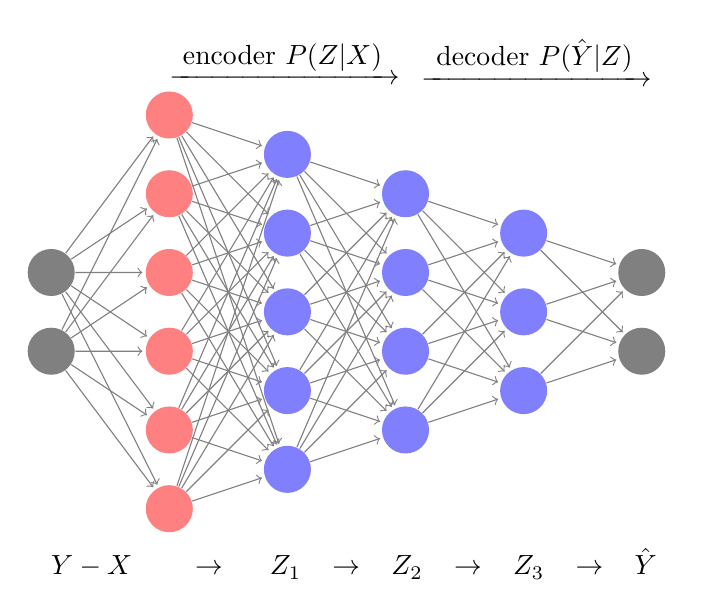
\begin{tikzpicture}[
	shorten >=1pt,->,draw=black!50, node distance=\layersep]
	\tikzstyle{every pin edge}=[<-,shorten <=1pt]
	\tikzstyle{neuron}=[circle,fill=black!25,minimum size=17pt,inner sep=0pt]
	\tikzstyle{source neuron}=[neuron, fill=black!50];
	\tikzstyle{output neuron}=[neuron, fill=black!50];
	\tikzstyle{data neuron}=[neuron, fill=red!50];
	\tikzstyle{hidden neuron}=[neuron, fill=blue!50];
	\tikzstyle{annot} = [text width=4em, text centered]
	
	% Draw source nodes
	\foreach \name / \y in {1,...,2}
	\node[source neuron] (I-\name) at (0,-\y-1.5) {};
	
	% Draw data nodes
	\foreach \name / \y in {1,...,6}
	\path[yshift=0.5cm]
	node[data neuron] (D-\name) at (\layersep,-\y cm) {};
	
	% Draw hidden 1 nodes
	\foreach \name / \y in {1,...,5}
	\path[yshift=0.5cm]
	node[hidden neuron] (H1-\name) at (\layersep*2,-\y-.5) {};
	
	% Draw hidden 2 nodes
	\foreach \name / \y in {1,...,4}
	\path[yshift=0.5cm]
	node[hidden neuron] (H2-\name) at (\layersep*3,-\y-1) {};
	
	% Draw hidden 3 nodes
	\foreach \name / \y in {1,...,3}
	\path[yshift=0.5cm]
	node[hidden neuron] (H3-\name) at (\layersep*4,-\y-1.5) {};
	
	% Draw output nodes
	\foreach \name / \y in {1,...,2}
	\node[output neuron] (O-\name) at (\layersep*5,-\y-1.5) {};
	
	% Connect source and data
	\foreach \source in {1,...,2}
	\foreach \dest in {1,...,6}
	\path (I-\source) edge (D-\dest);
	
	% Connect data and hidden 1
	\foreach \source in {1,...,6}
	\foreach \dest in {1,...,5}
	\path (D-\source) edge (H1-\dest);
	
	% Connect hidden 1 and 2
	\foreach \source in {1,...,5}
	\foreach \dest in {1,...,4}
	\path (H1-\source) edge (H2-\dest);
	
	% Connect hidden 2 and 3
	\foreach \source in {1,...,4}
	\foreach \dest in {1,...,3}
	\path (H2-\source) edge (H3-\dest);
	
	% Connect every node in the hidden layer with the output layer
	\foreach \source in {1,...,3}
	\foreach \dest in {1,...,2}
	\path (H3-\source) edge (O-\dest);
	
	% Annotate
	\node[text width=6cm] at (4.5,0.16){$\xrightarrow{\makebox[2.7cm]{encoder $P(Z\vert X)$}}$};
	\node[text width=1cm] at (5.2,0.18){$\xrightarrow{\makebox[2.7cm]{decoder $P(\hat{Y}\vert Z)$}}$};
	\node[text width=8cm] at (4,-6.2) {$Y-X\hspace{.7cm}\rightarrow\hspace{.5cm}Z_1\hspace{.3cm}\rightarrow\hspace{.3cm}Z_2\hspace{.3cm}\rightarrow\hspace{.3cm}Z_3\hspace{.3cm}\rightarrow\hspace{.3cm}\hat{Y}$};
\end{tikzpicture}
}
\caption{The layers form a Markov chain of successive internal representations.}
\end{figure}

The $k$ layers of a DNN form a Markov chain ${Y \rightarrow X \rightarrow Z_1 \rightarrow \ldots \rightarrow Z_k \rightarrow \hat{Y}}$ of successive representations $\{Z_i:i=1,\ldots,k\}$. Each representation $Z_i$ of the $i$-th hidden layer is a single multivariate random variable. The Markov chain satisfies the DPI (\ref{eq:dpi}):
\begin{align}
I(X;Y) \geq I(Z_1;Y) \geq I(Z_2;Y) \geq \ldots \geq I(Z_k;Y) \geq I(\hat{Y};Y),\\
H(X) \geq I(X;Z_1) \geq I(X;Z_2) \geq \ldots \geq I(X;Z_k) \geq I(X;\hat{Y}).
\end{align}
A DNN is designed to learn how to describe $X$ to predict $Y$ and eventually, to compress $X$ to only hold the information related to $Y$. Tishby describes this processing as ``successive refinement of relevant information''.

\subsection*{Information Plane}

Given $P(X;Y)$, $Z$ is uniquely mapped to a point in the \emph{information plane} with coordinates $(I(X;Z),I(Z,Y))$. Since layers related by invertible re-parametrization (\ref{eq:repara}) appear in the same point, each information path in the plane corresponds to many different networks, with possibly very different architectures. The layers are mapped to $k$ monotonic connected points in the plane. This unique \emph{information path} satisfies the DPI chains.

The decoder mutual information $I(Z;Y)$ corresponds to the \emph{generalization error} or out of sample error. The encoder mutual information $I(X;Z)$ corresponds to the \emph{sample complexity} or number of samples required achieve some accuracy.

\subsection*{Network and Data}

We train a deep neural network with fully-connected topology of layer sizes 12-10-8-6-4-2-1 neurons and with hyperbolic tangent function, shifted to a sigmoidal function in the final layer. The networks were trained using SGD and the cross-entropy loss function, with no other explicit regularization.
The data is \emph{12 binary inputs} that represent 12 uniformly distributed points on a 2D sphere. With such rules, the 4,096 different patterns of the input variable X are divided into 64 disjoint orbits of the rotation group. These orbits form a minimal sufficient partition/statistics for spherically symmetric rules.

\subsection*{Computing Mutual Information}

Estimating the mutual information of the layers in a Neural Network is done by estimating the probability density from a finite number of samples. Assume that we have a number $N$ of samples in the training set and the probability density $P(X)$, $P(Z\vert X)$ and $P(X,Y)$ are approximated by counting the number of cases with the values of the variables belonging to a \emph{discretized interval}.

\subsection*{Findings}

We define a deep neural network (DNN) as a Markov chain and study the information paths of its hidden layers in the information plane spanned by the two order parameters $I(Z;X)$ and $I(Z;Y)$. This is feasible if $P(X,Y$) is known and $P(Z \vert X)$ and $P(Y\vert Z)$ are tractable (or can be estimated). The main findings are:
\begin{enumerate}
	\item \emph{Dynamics of SGD:} We observe a phase transition from fast drift (ERM) to random diffusion or stochastic relaxation (compression) constrained by the training error when the training errors becomes small. Most of the epochs are spent on compression, not fitting the labels.
	\item \emph{Optimal representations:} The converged layers lie very close to the Information Bottleneck theoretical bound. This generalization through noise mechanism is unique to deep networks and absent in one layer networks.
	\item \emph{Benefits of the hidden layers:} The training time is dramatically reduced when adding more hidden layers. Thus the main advantage of the hidden layers is computational. This can be explained by the reduced relaxation time, as this it scales super-linearly (exponentially for simple diffusion) with the information compression from the previous layer.
	\item \emph{Benefits of sample size:} With increased sample size, the decoder mutual information is pushed up and gets closer to the theoretical information bottleneck bound. It is the mutual information, not the layer size or VC dimension, that determines generalization, different from standard theories.
\end{enumerate}

\subsection*{Finding 1: Dynamics of Stochastic Gradient-Descent}

When depicting the dynamics of Stochastic Gradient-Descent (SGD) on the information plane over epochs, we observe a phase transition between a short drift (i.e. ERM) and a long random diffusion (i.e. compression) phase:

\begin{enumerate}
\item \emph{Drift Phase:} The layers increase the information on the labels, $I(Z;Y)$, while preserving the DPI order (lower layers have higher information), i.e., ERM.
\item \emph{Diffusion Phase:} The layers information on the input, $I(X;Z)$, decreases and the layers lose irrelevant information until convergence, i.e., compression.
\end{enumerate}

First, in the drift phase, the decoder mutual information $I(Z;Y)$ increases which results in a decreased generalization error (accuracy increases). Second, in the diffusion phase, the encoder mutual information $I(X;Z)$ decreases as the hidden layers compress the information and ``forget'' some information. Tishby believes that \emph{``the most important part of learning is actually forgetting''}.

\begin{figure}[H]
\centering
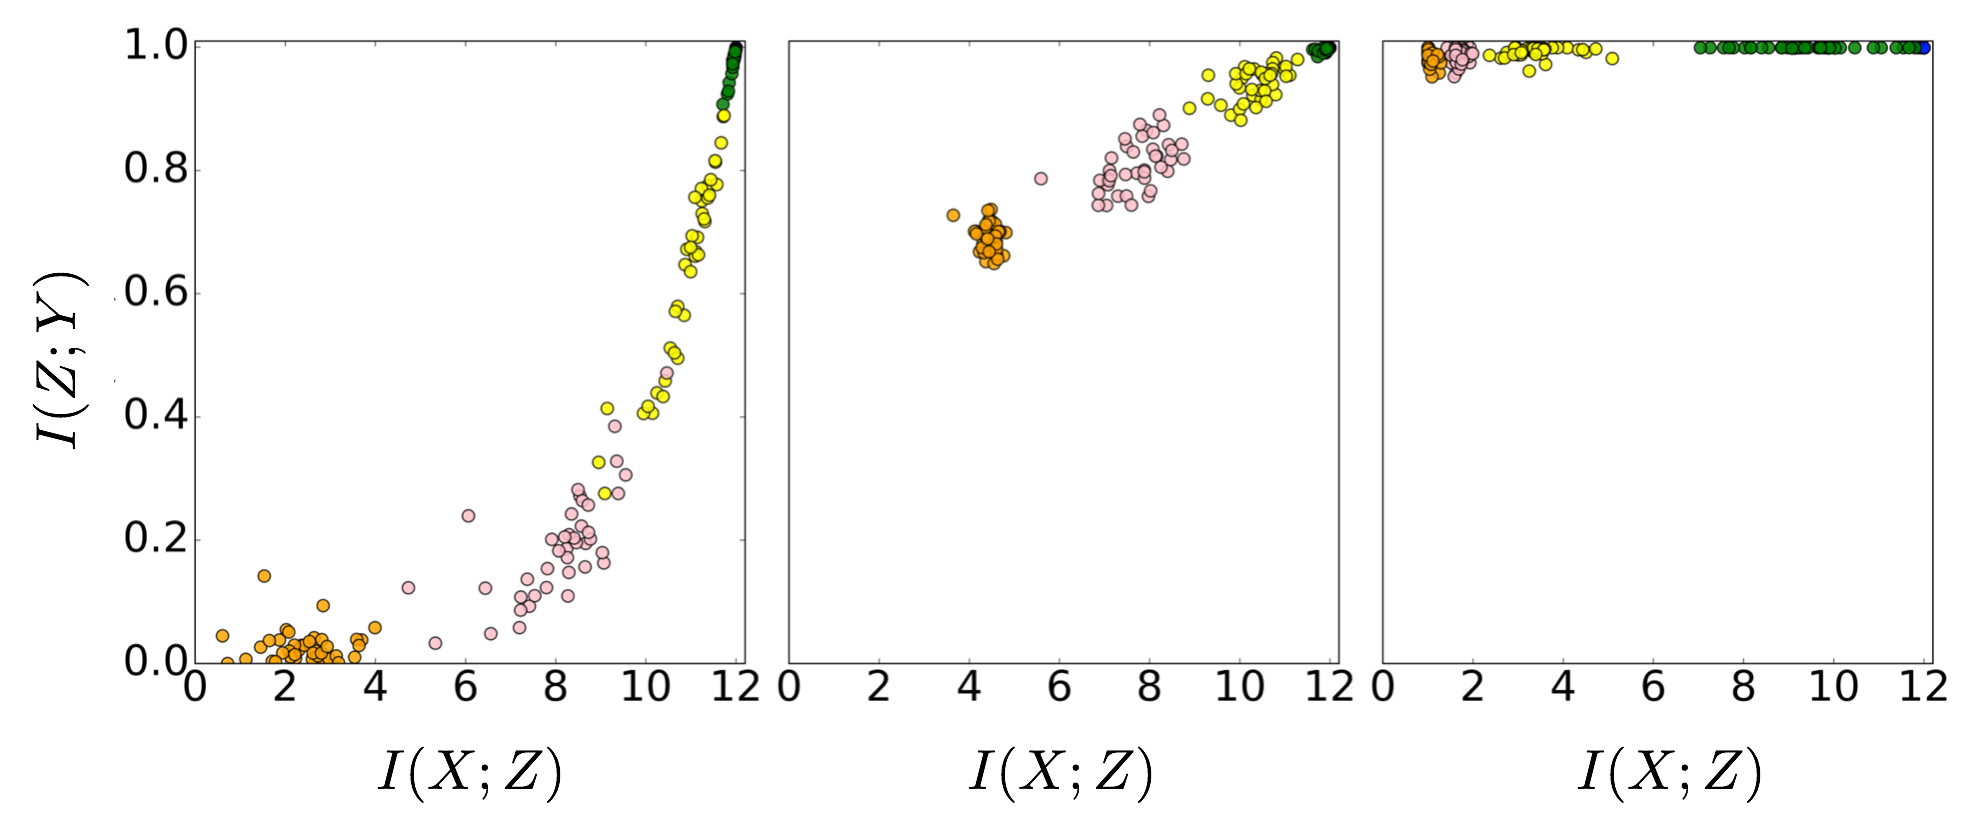
\includegraphics[width=0.9\textwidth]{plane}
\caption{Three snapshots the encoder $I(X;Z)$ and decoder $I(Z;Y)$ mutual information of the layers of 50 randomized networks during the SGD optimization process in the information plane (in bits): \emph{left:} 1 epoch, \emph{center:} 400 epochs, \emph{right:} 9,000 epochs. Layers in green being the closest to input $X$, layers in orange being the furthest away. }
\end{figure}

We can observe the phenomena in the behavior of the weight gradients $\nabla W_i$. In the drift phase $I(Z;Y)$ increases quickly as the empirical error decreases. The gradient means are much smaller than their standard deviations. In the diffusion phase, the gradients means are very small compared to their batch to batch fluctuations.

\begin{figure}[H]
	\centering
	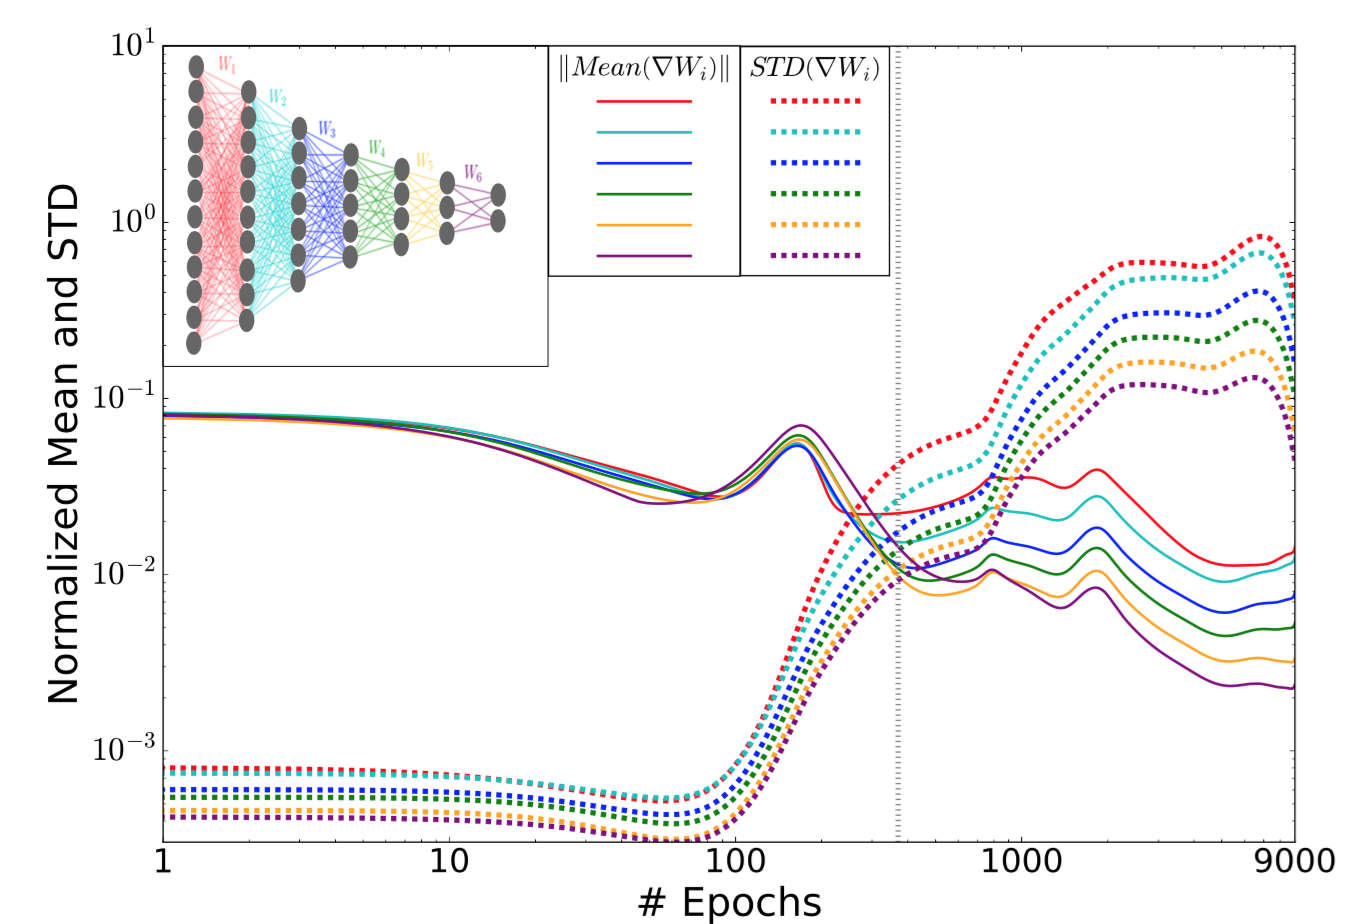
\includegraphics[width=0.7\textwidth]{gradient}
	\caption{Mean $\rVert Mean(\nabla W_i)\rVert_2$ (filled line) and standard deviation $STD(\nabla W_i)$ (dotted line) of stochastic gradient $\nabla W_i$. The grey line ($\sim350$ epochs) marks the transition between the first phase, with large gradient means and small variance (drift, high gradient SNR), and the second phase, with large fluctuations and small means (diffusion, low SNR).}
\end{figure}

While the increase of $I(Z;Y)$ in the ERM phase is expected from the cross-entropy loss minimization, the surprising compression phase requires an explanation. There was no explicit regularization that could simplify the representations. The diffusion phase mostly adds random noise to the weights, and they evolve like Wiener processes, under the constraint of the training error. Such diffusion processes can be described by the Fokker-Planck equation, whose stationary distribution maximizes the entropy of the weights distribution, under the training error constraint. This maximizes $H(X\vert Z_i)$, or minimizes $I(X;Z_i) = H(X) - H(X\vert Z_i)$, because the input entropy $H(X)$ remains constant. This entropy maximization by additive noise, also known as \emph{stochastic relaxation}, is constrained by the empirical error. By minimizing $I(X;Z_i)$ for each layer $i$, the diffusion phase leads to more compressed representations.

\subsubsection*{From Stochastic Gradient-Descent to Ornstein-Uhlenbeck Process}

Consider an objective function of the form $\mathcal L(\theta) = \sum_{n=1}^N l_n(\theta)$. Let $S(t)$ be a set of indices drawn uniformly at random from set $\{1,2,\dots,N\}$. We can form a stochastic estimate of the objective and a stochastic gradient,
\begin{align}
\hat L(\theta) &= \frac{N}{S} \sum_{n\in S} l_n(\theta),\\
\hat g_s(\theta) &= \nabla_\theta  \hat L(\theta).
\end{align}
In expectation, the stochastic gradient is the full gradient, $g(\theta) = \mathbb E(\hat{g}_s(\theta) )$. The stochastic gradient is used for the update:
\begin{equation}
\theta(t+1) = \theta(t) - \hat\epsilon \hat g_S(\theta(t)).
\end{equation}
To approximate SGD with a continuous time process, some assumptions are made:
\begin{itemize}
\item[1.] Assume that the gradient noise $\hat g_S(\theta)-g(\theta) $ is Gaussian distributed.
\item[2.] Assume that the iterates $\theta(t)$ are constrained to a small enough region in parameter space that the sampling noise covariance of the stochastic gradients is constant.
\item[3.] Assume that the step size is small enough so that we can approximate the discrete-time Markov chain defined by SGD with a continuous-time Markov process.
\end{itemize}

Based on assumption 1, if S is big enough, then the central limit theorem should apply and we can write the stochastic gradient as
\begin{equation}
\hat g_S(\theta) \approx g(\theta) + \hat \xi_S(\theta), \quad \hat \xi_S(\theta)\sim \mathcal N(0,C(\theta)/S).
\end{equation}
Decompose the covariance matrix C into $C = BB^T$, we introduce a rescaled noise covariance matrix $B_{\epsilon/S} = \sqrt{\epsilon/S}B$. And according to assumption 2 we can relax B to a constant irrelevant to $\theta$.
Then 
\begin{equation}
\theta(t+1) - \theta(t) = -\epsilon g(\theta(t) + \sqrt{\epsilon} B_{\epsilon/S}W(t), \quad W(t)\sim \mathcal N(0,I).
\end{equation}
In the continuous version is 
\begin{equation}
d\theta(t) = -\nabla_\theta \mathcal L (\theta)dt + B_{\epsilon/S} dW(t).
\end{equation}
As we want $\theta(t)$ to be close to the stationary point when $d\theta(t)$ is small, where the noise dominates the gradient. So we need a further assumption on the gradient, that is 

\begin{itemize}
\item[4.] Assume that the stationary distribution of the iterates is constrained to a region within which the objective is well approximated by a quadratic function. 
\end{itemize}
Now we can write the $\nabla_\theta \mathcal L (\theta)$ explicitly as 
\begin{equation}
d\theta(t) = -A(\theta(t)-\hat \theta)dt + B_{\epsilon/S} dW(t).
\label{eq:sde}
\end{equation}
The solution of SDE (\ref{eq:sde}) is identified as a multidimensional Ornstein-Uhlenbeck process. The probability density function of the Ornstein-Uhlenbeck process satisfies the Fokker-Planck equation.

\subsection*{Finding 2: Optimal Representation}

\myworries{write}

\subsection*{Finding 3: Benefits of the Hidden Layers}

The hidden layers can be understood of a computational means reducing the stochastic relaxation phase.

\begin{figure}[H]
	\centering
	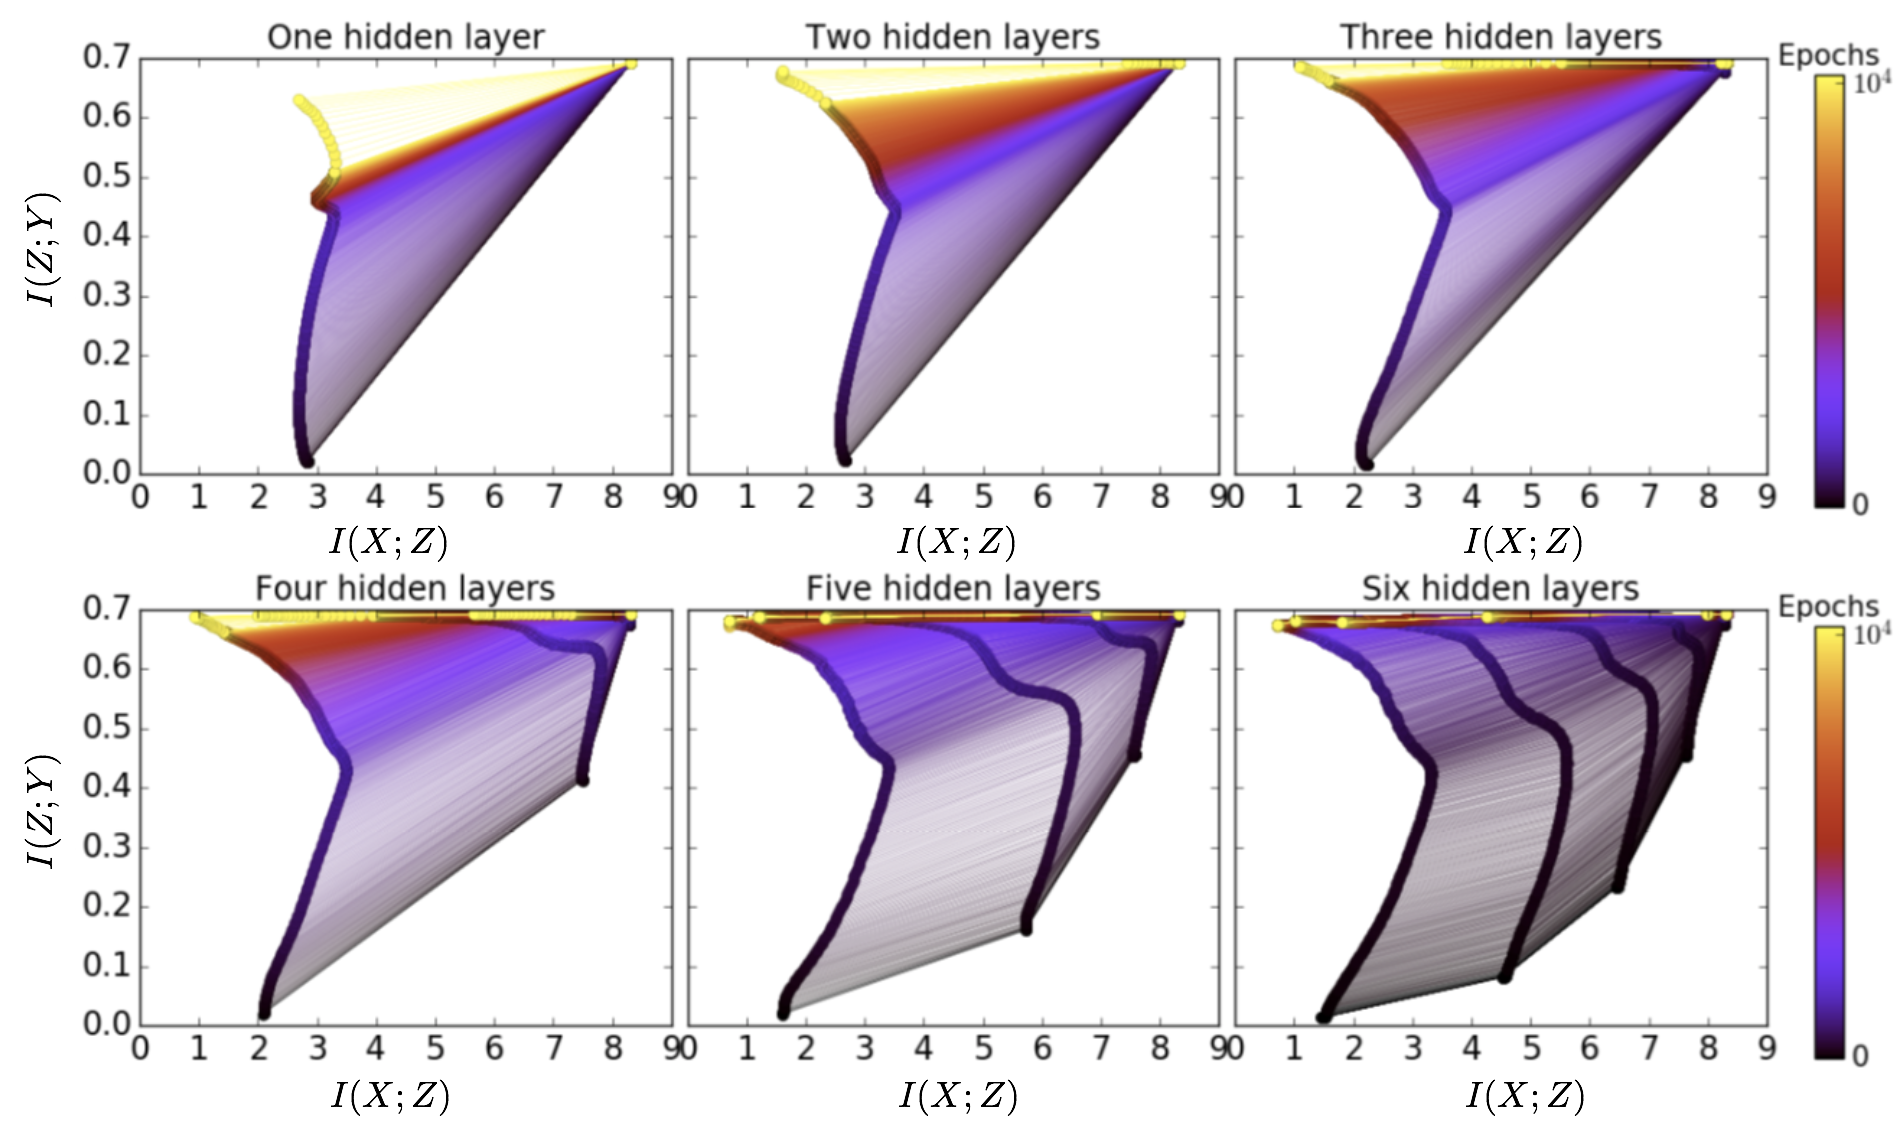
\includegraphics[width=0.9\textwidth]{layers}
	\caption{Hidden layers shorten the training time in the diffusion phase.}
\end{figure}

In one spatial dimension $x$, for an Ito process driven by the standard Wiener process $W_t$ and described by the SDE
\begin{equation}
dX_t = \mu(X_t, t) \,dt + \sigma(X_t, t) \,dW_t
\end{equation}
with drift velocity  $\mu(X_t, t)$ and diffusion coefficient $D(X_t, t) = \sigma^2(X_t, t)/2$, the Fokker–Planck equation for the probability density $p(x, t)$ of the random variable $X_t$ is
\begin{equation}
\frac{\partial}{\partial t} p(x, t) = -\frac{\partial}{\partial x}\left[\mu(x, t) p(x, t)\right] + \frac{\partial}{\partial x}D(x, t)\frac{\partial}{\partial x}p(x, t).
\label{fokker}
\end{equation}
Then, according to the diffusion equation (\ref{fokker}), the relaxation time of layer $k$ is proportional to the exponential of this layer's compression amount $\Delta S_k:\Delta t_k\sim \exp(\Delta S_k)$. We can compute the layer compression as $\Delta S_k = I(X;Z_k)-I(X;Z_{k-1})$. Because $\exp(\sum_k \Delta S_k) \geq \sum_k \exp(\Delta S_k)$, we would expect an \emph{exponential decrease in the training epochs} with increasing number of hidden layers $k$.

\subsection*{Finding 4: Benefit of Sample Size}

Fitting more training data requires more information captured by the hidden layers. With increased training data size, the decoder mutual information (recall that this is directly related to the generalization error), $I(Z;Y)$, is pushed up and gets closer to the theoretical information bottleneck bound.

\begin{figure}[H]
	\centering
	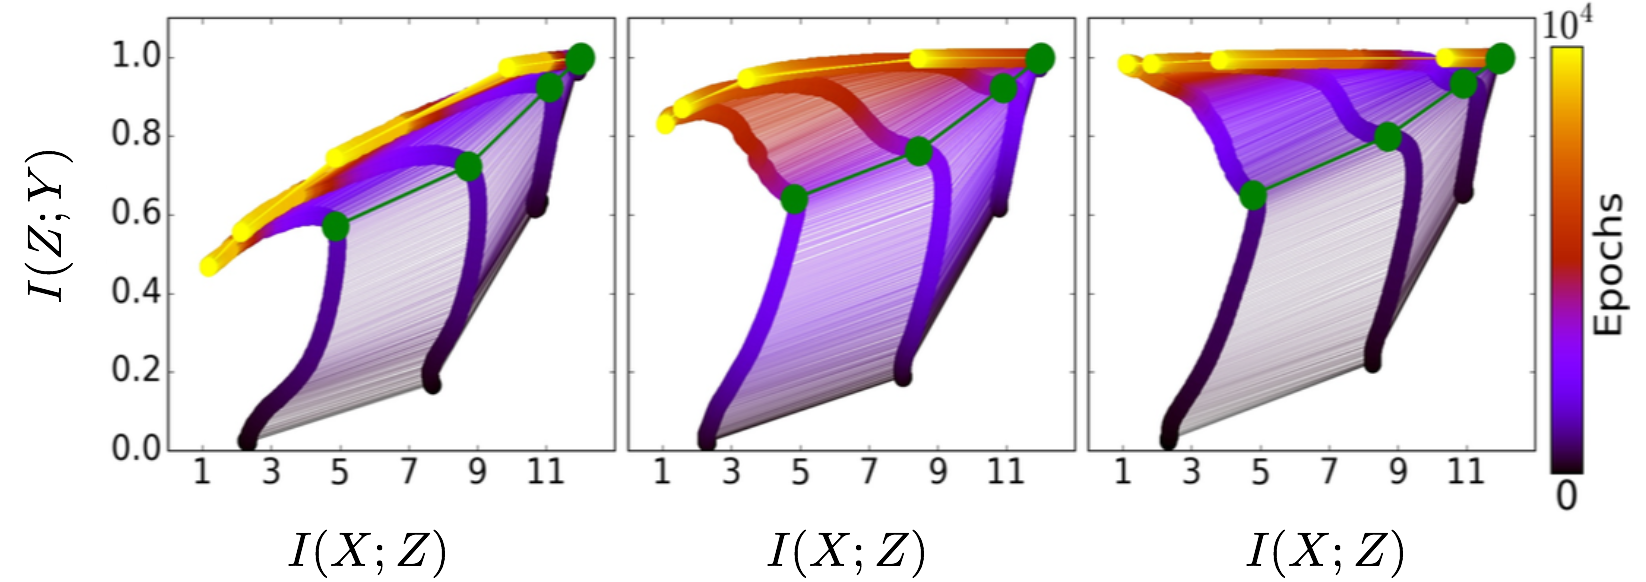
\includegraphics[width=0.9\textwidth]{sample}
	\caption{The green line indicates SGD drift-diffusion phase transition with respect to sample size: \emph{left:} 5\% data, \emph{center:} 45\% data epochs, \emph{right:} 85\% data.}
\end{figure}

Tishby emphasized that it is the \emph{mutual information, not the layer size or the VC dimension, that determines generalization}, different from standard theories.

\section{Learning Theory}

\subsection*{``Old'' Generalization Bounds}

The generalization bounds defined by classic learning theory is:
\begin{equation}
\epsilon^2 < \frac{\log \vert H_\epsilon \vert + \log 1/\delta}{2m}
\label{eq:bound}
\end{equation}
where
\begin{itemize}
	\item[-] $\epsilon$: The difference between training and generalization error.
	\item[-] $H_\epsilon$: $\epsilon$-cover of the hypothesis class, typically, we assume $\vert H_\epsilon \vert\sim (1/\epsilon)^d$.
	\item[-] $\delta$: Confidence.
	\item[-] $m$: The number of training samples.
	\item[-] $d$: The VC dimension of the hypothesis.
\end{itemize}

The bound (\ref{eq:bound}) states that the difference between the training error and the generalization error is bounded by a function of the hypothesis space size and the dataset size. The larger the hypothesis space gets, the bigger the generalization error becomes.

However, it does not work for deep learning. The larger a network is, the more parameters it needs to learn. With this generalization bounds, \emph{larger networks (larger $d$) would have worse bounds}. This is contrary to the intuition that larger networks are able to achieve better performance with higher expressivity.

\subsection*{``New'' Input Compression Bounds}

To solve this counterintuitive observation, Tishby et al. proposed a new input compression bound for DNN.

First, let us have $Z_\epsilon$ as an $\epsilon$-partition of the input variable $X$. This partition compresses the input with respect to the homogeneity of the labels into small cells. The cells in total can cover the whole input space. If the prediction outputs binary values, we can replace the cardinality of the hypothesis, $\vert H_\epsilon\vert$, with $2^{\vert Z_\epsilon\vert}$.
\begin{equation}
\vert H_\epsilon\vert \sim 2^{\vert X \vert} \rightarrow 2^{\vert Z_\epsilon\vert}.
\end{equation}
When $X$ is large, the size of $X$ is approximately $2^{H(X)}$. Each cell in the $\epsilon$-partition is of size $2^{H(X\vert Z_\epsilon)}$. Therefore, we have $\vert Z_\epsilon\vert\sim \frac{2^{H(X)}}{2^{H(X\vert Z_\epsilon)}} = 2^{I(Z_\epsilon;X)}$. Then, the input compression bound becomes:
\begin{equation}
\epsilon^2 < \frac{2^{I(Z_\epsilon;X)}+\log 1/\delta}{2m}.
\end{equation}

\section{Variational Bottleneck}

\subsection*{Variational Formulation}

\myworries{write}

\subsection*{From Information Bottleneck to Variational Autoencoder}

The information bottleneck objective is finding the statistic $Z(X)$ that is sufficient $I(X;Y) = I(Z;Y)$ with minimal $I(X;Z)$:
\begin{align}
\min &\quad I(X; Z)\\
s.t. &\quad I(Z;Y)=I(X;Y).
\end{align}
We relax the formulation into the information bottleneck lagrangian:
\begin{equation}
\mathcal{L} =  I(X; Z) -\beta I(Z;Y),\quad\beta>0.
\label{eq:ib_lag}
\end{equation}
Let $P_\theta(Z\vert X)$ and $P_\theta(Y\vert Z)$ denote variational approximations parameterized by $\theta$. We can rewrite the two terms of (\ref{eq:ib_lag}) as:
\begin{align}
I(Z;Y) &\simeq \E_{x,y\sim P(X,Y)} \left[ \E_{z\sim P_\theta(Z\vert X)}[-\log p_\theta(y\vert z)] \right],\\
I(X; Z) &= \E_{x\sim P(X)}\left[ D_{KL}(p_\theta(z\vert x) \rVert p_\theta(z)) \right].
\end{align}
Given training set $\{(x_i,y_i):i=1\ldots,N\}\sim P(X,Y)$, we approximate (\ref{eq:ib_lag}) empirically as
\begin{equation}
\mathcal{L}(\theta) = \frac{1}{N}\sum_{i=1}^N \E_{z\sim p_\theta(Z\vert X=x_i)}[-\log p_\theta(y_i\vert z)] + \beta D_{KL}(p_\theta(z\vert x_i) \rVert p_\theta(z)).
\label{eq:ib_approx}
\end{equation}
In an unsupervised regime, the task is reconstruction $y=x$ and (\ref{eq:ib_approx}) reduces to:
\begin{equation}
\mathcal{L}(\theta) = \frac{1}{N}\sum_{i=1}^N \E_{z\sim p_\theta(Z\vert X=x_i)}[-\log p_\theta(x_i\vert z)] + \beta D_{KL}(p_\theta(z\vert x_i) \rVert p_\theta(z)).
\label{eq:ib_unsup}
\end{equation}
In fact, for $\beta=1$ we obtain the objective of the variational auto-encoder (VAE). For arbitrary $\beta$, this is precisely the objective formulation the $\beta$-VAE .

\begin{proof}
\myworries{rewrite}
Consider the information bottleneck objective in an unsupervised setting:
\begin{equation}
\max I(Z;X) - \beta I(Z;i).
\label{eq:ib_unsuper}
\end{equation}
Then, bound the first term
\begin{align}
I(Z;X) 
&= \iint dx\,dz\,p(x,z) \log p(x|z)/p(x) \\
&= H(x) + \iint dx\,dz\,p(x,z) \log p(x|z)  \\
&= H(x) + \int dz\,p(z) \int dx\,p(x|z) \log p(x|z)  \\
&\geq \int dz\,p(z) \int dx\,p(x|z) \log q(x|z) \label{eq:kl_pos} \\
&= \iint dx\,dz\,p(x,z) \log q(x|z)  \\
&= \int dx\,p(x) \int dz\,p(z|x) \log q(x|z).
\end{align}
where in (\ref{eq:kl_pos}) we dropped $H(X)$ and used the non-negativity of the Kullback-Leibler divergence $D_{KL}(p(x\vert z)\rVert q(x\vert z)) \geq 0$ to substitute intractable $p(x\vert z)$ by variational decoder $q(x\vert z)$.
For the second term, note:
\begin{equation}
p(z\vert i) = \int dx\,p(z\vert x)p(x\vert i) = \int dx\,p(z\vert x)\delta(x-x_i) = p(z\vert x_i),
\end{equation}
and take $p(i) = 1/N.$
Then, bound the second term from above
\begin{align}
I(Z,i)
&= \sum_i\int dz\,p(z\vert i)p(i)\log\frac{p(z\vert i)}{p(z)}\\
&= \frac{1}{N} \sum_i\int dz\, p(z\vert x_i)\log\frac{p(z\vert x_i)}{p(z)}\\
&\leq \frac{1}{N} \sum_i\int dz\, p(z\vert x_i) \log\frac{p(z\vert x_i)}{r(z)}\label{eq:marginal},
\end{align}
where in (\ref{eq:marginal}) we replace the intractable $p(z)$ by variational marginal $r(z)$.
When applying both bounds to (\ref{eq:ib_unsuper}) the objective takes the form
\begin{equation}
I(Z;X) - \beta I(Z;i) \leq \int dx\,p(x)\int dz\, p(z\vert x) \log q(x\vert z) - \beta \frac{1}{N} \sum_i D_{KL}(p(Z\vert x_i)\rVert r(Z)),
\end{equation}
\end{proof}

\end{document}
